\documentclass[letterpaper,12pt]{article}
\usepackage[utf8]{inputenc}
\usepackage{fullpage}
\usepackage{courier}
\usepackage[margin=0.75in]{geometry}
\usepackage{listings}
\usepackage{color}
\usepackage{graphicx}
\usepackage[width=5in]{caption}
\usepackage{hyphenat}

% Format a sectionless paragraph
\newcommand*\unparagraph{
	\par
	\nopagebreak
	\vskip3.25ex plus1ex minus.2ex
	\noindent
}

% define extra colors
\definecolor{dkgreen}{rgb}{0,0.6,0}
\definecolor{purple}{RGB}{159,0,197}

% define the code listing format
\lstset{
	language=C++,
	basicstyle=\footnotesize\ttfamily,
	backgroundcolor=\color{white},
	showspaces=false,
	showstringspaces=false,
	frame=none,
	tabsize=3,
	keywordstyle=\color{purple},
	commentstyle=\color{dkgreen},
	stringstyle=\color{blue},
	escapeinside={\%*}{*)}
}

% efine the title/header
\title{\Large CS 3468\\Lab 2} 
\author{Jared Wallace}
\date{}

\begin{document}

\maketitle

\vspace{30mm}

\section*{Objectives}
\begin{enumerate}
\item Understand the design of a sensor application
\item Begin to learn component-based programming languages
\end{enumerate}

\section*{Tasks}
\begin{enumerate}
\item \textbf{Architecture and concepts of a sensor application}
    All of our work will be done in nesC, which is just C with some extra features.
    A nesC application consists of one or more \emph{Components} assembled, or \emph{wired},
    to form an application executable. Components define two scopes: one for
    their specification which contains the names of their \emph{interfaces},
    and a second scope for their implementation. A component \emph{provides} and \emph{uses}
    interfaces. The provided interfaces are intended to represent the
    functionality that the component provides to its user in its specification;
    the used interfaces represent the functionality the component needs to
    perform its job in its implementation.

    Interfaces are bidirectional: they specify a set of \emph{commands}, which
    are functions to be implemented by the interface's provider, and a set of
    \emph{events}, which are functions to be implemented by the interface's user.
    \begin{itemize}
        \item For a component to call the commands in an interface, it must
              implement the events of that interface.
        \item A single component may use or provide multiple interfaces and
              multiple instances of the same interface.
        \item The set of interfaces which a component provides,
              together with the set of interfaces that a component uses,
              is considered that component's \emph{signature}. 
    \end{itemize}

    There are two types of components: \emph{configuration} and \emph{module}.
    \begin{itemize}
        \item Modules provide the implementations of one or more interfaces.
        \item Configurations are used to assemble other components together,
              connecting interfaces used by components to interfaces provided
              by others.
        \item Every nesC application is described by a top-level configuration
              that wires together the components inside. 
    \end{itemize}

   A module is the basic unit that provides the functions of the application.
   \begin{itemize}
      \item A module must implement every command of the interfaces it \textbf{provides}, and every event of the interfaces it \textbf{uses}.
      \item A configuration has no implementation, but rather sub-components and wirings.
      \item A module has no sub components or wirings, but rather an implementation.
   \end{itemize}

   All of the concepts (in italics), and the hierarchical application architecture, are actually reflected in the programming language (which we will learn next).

\item \textbf{Source files of a sensor application}
   A sensor application has at least three files: a configuration file, a module file and a Makefile.
   Both the configuration and the module files have the extension “.nc”.

   \begin{enumerate}
      \item The top component of our example application is called "BlinkAppC".
         The configuration file is named “BlinkAppC.nc”. That file declares that the application needs four components, to wit: MainC, BlinkC, LedsC and TimerC.
         \begin{lstlisting}
         configuration BlinkAppC {
         }
         implementation {
           components MainC, BlinkC, LedsC;
           components new TimerMilliC() as TimerC;

           BlinkC.Boot -> MainC.Boot;
           BlinkC.Timer -> TimerC.Timer;
           BlinkC.Leds -> LedsC.Leds;
         }
         \end{lstlisting}
         \begin{itemize}
             \item \emph{MainC} (provided by TinyOS) is the entry of the sensor application. It must be included in every sensor application (just like the main() function must be included in a C program).
             \item \emph{BlinkC} (made by you) is the actual component that controls the blinks.
             \item \emph{LedsC} (provided by TinyOS) is the component that controls the LEDs.
             \item \emph{TimerC} (provided by TinyOS) is the timing component.
         \end{itemize}
         Components are connected via interfaces. A connection between components means a component uses an interface provided by another component.
         In this application, BlinkC uses the Boot interface provided by MainC, as well as the Timer interface provided by TimerC and the Led interface provided by LedsC. (All interfaces are defined by TinyOS)
         \begin{itemize}
            \item The \emph{Boot} interface provides the \emph{booted()} event that notifies connected components when the Mainc component has finished initialization.
            \item The \emph{Timer} interface provides the \emph{fired()} event that notifies connected components when the timing component completes the countdown to 0.
            \item The \emph{Leds} interface provides a few commands to turn on or off LEDs on the mote.
         \end{itemize}
         Now, read through the file “BlinkAppC.nc” until you understand what components are used in the application, and how they are connected.

      \item The MainC, LedsC and TimerC components are already implemented in system libraries.
         Only the BlinkC component needs to be programmed in the application.
         (The implementation is in the file “BlinkC.nc”)
         It declares the BlinkC to be a module using three interfaces.

         \begin{lstlisting}
         module BlinkC {
           uses interface Timer<TMilli> as Timer;
           uses interface Leds;
           uses interface Boot;
         }
         \end{lstlisting}

         Recall that a module \textbf{must} implement every command of interfaces it provides, and every event of interfaces it uses.
         Accordingly, BlinkC needs to implement the booted() event (since it uses the Boot interface), and needs to implement the fired() event (as it uses the Timer interface).
         BlinkC does not need to implement any commands, as it does not provide any interface.

         Now, read through the file “BlinkC.nc” until you understand how the module is implemented, how the module calls commands in other components, and what the module does upon an event.
      \item The Makefile always takes the format shown below. (The first line indicates the top component of the application)
         \begin{lstlisting}
            COMPONENT=BlinkAppC
            include $(MAKERULES)
         \end{lstlisting}
         Now, compile and run the application and verify that what you see matches the application code.
\end{enumerate}
   \item Make a new Blink application so that LEDs blink as a counter
      Requirements:
      \begin{itemize}
         \item LED \textbf{off} means 0, and LED \textbf{on} means 1.
         \item The three LEDs encode a 3-bit number.
         \item The application generates a counting sequence of 3-bit \textbf{gray codes} as 0 1 3 2 6 7 5 4.
         \item The counting should have a frequency of 1 number per second.
      \end{itemize}
\end{enumerate}
\section*{Lab Report}
\begin{enumerate}
   \item Please demonstrate your program to the lab instructor and let him check your code at the end of the current lab project.
   \item Your project report is due at the beginning of the next lab.
   \item Grading criteria
      \begin{itemize}
         \item Demonstration, 15 percent
         \item Code, 15 percent
         \item Report, 70 percent
      \end{itemize}
\end{enumerate}
\section*{Report instructions}
Format:
\begin{enumerate}
   \item Include your name and ID in the first page
   \item Font size of at least 10pt
   \item Single spaced
   \item Maximum of 5 pages (I will take points off for exceeding this without any good reason)
   \item Please submit as PDF online, and turn in a hard copy
\end{enumerate}
Content:
\begin{enumerate}
   \item Introduction (10 percent of the report grade) Please summarize the task of this lab and what you have learned in the lab
   \item Implementation (30 percent of the report grade) Please describe in detail how your made your program. Show what components you used, how they are wired, and through what interfaces.
   \item Experiment (30 percent of the report grade) Please describe in detail what can be observed from your program and explain how said observed behavior is a result of your code (and not happy coincidence).
\end{enumerate}

% Comic at the bottom
\begin{figure}[ht!]
	\centering
	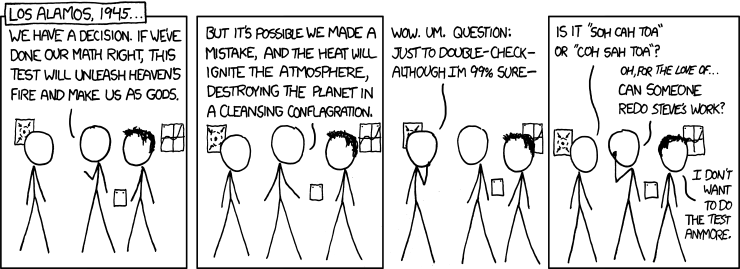
\includegraphics[width=5in]{los_alamos.png}
   \caption*{The test didn't (spoiler alert) destroy the world, but the fact that they were even doing those calculations makes theirs the coolest jobs ever.}
\end{figure}

\end{document}
